
\documentclass{article}
\usepackage{graphicx}
\usepackage{indentfirst}
\usepackage[margin=1.5in]{geometry}

\begin{document}
\title{Spécifiation des exigences du modèle : Jalon 3}

\author{Louis-Vincent CAPELLI \and Alexandre THEISSE \and Tom SARTORI \and Raphaël TURCOTTE}
\date{\today}
\maketitle
\newpage

\tableofcontents
\newpage

\section{Introduction}
\subsection*{Objet et portée du document}
Ce document a pour but de spécifier les exigences du jalon 3 du projet "Système
de surveillance de la qualité de l'air" (SSQA). Il est destiné aux membres du 
groupe de travail, afin de leur permettre de cerner correctement les besoins
du client et de les retranscrire lors de la conception.

\section{Présentation}
\subsection{Mise en contexte}
Lors du jalon 1, le schéma préliminaire de la base de données a été
modifié afin de mieux correspondre aux besoins du client. Le schéma a ensuite
été légèrement modifié lors du jalon 2 à des fins de correction, résultant
en un schéma final qui est présenté ci-dessous.

\begin{figure}[h]
    \centering
    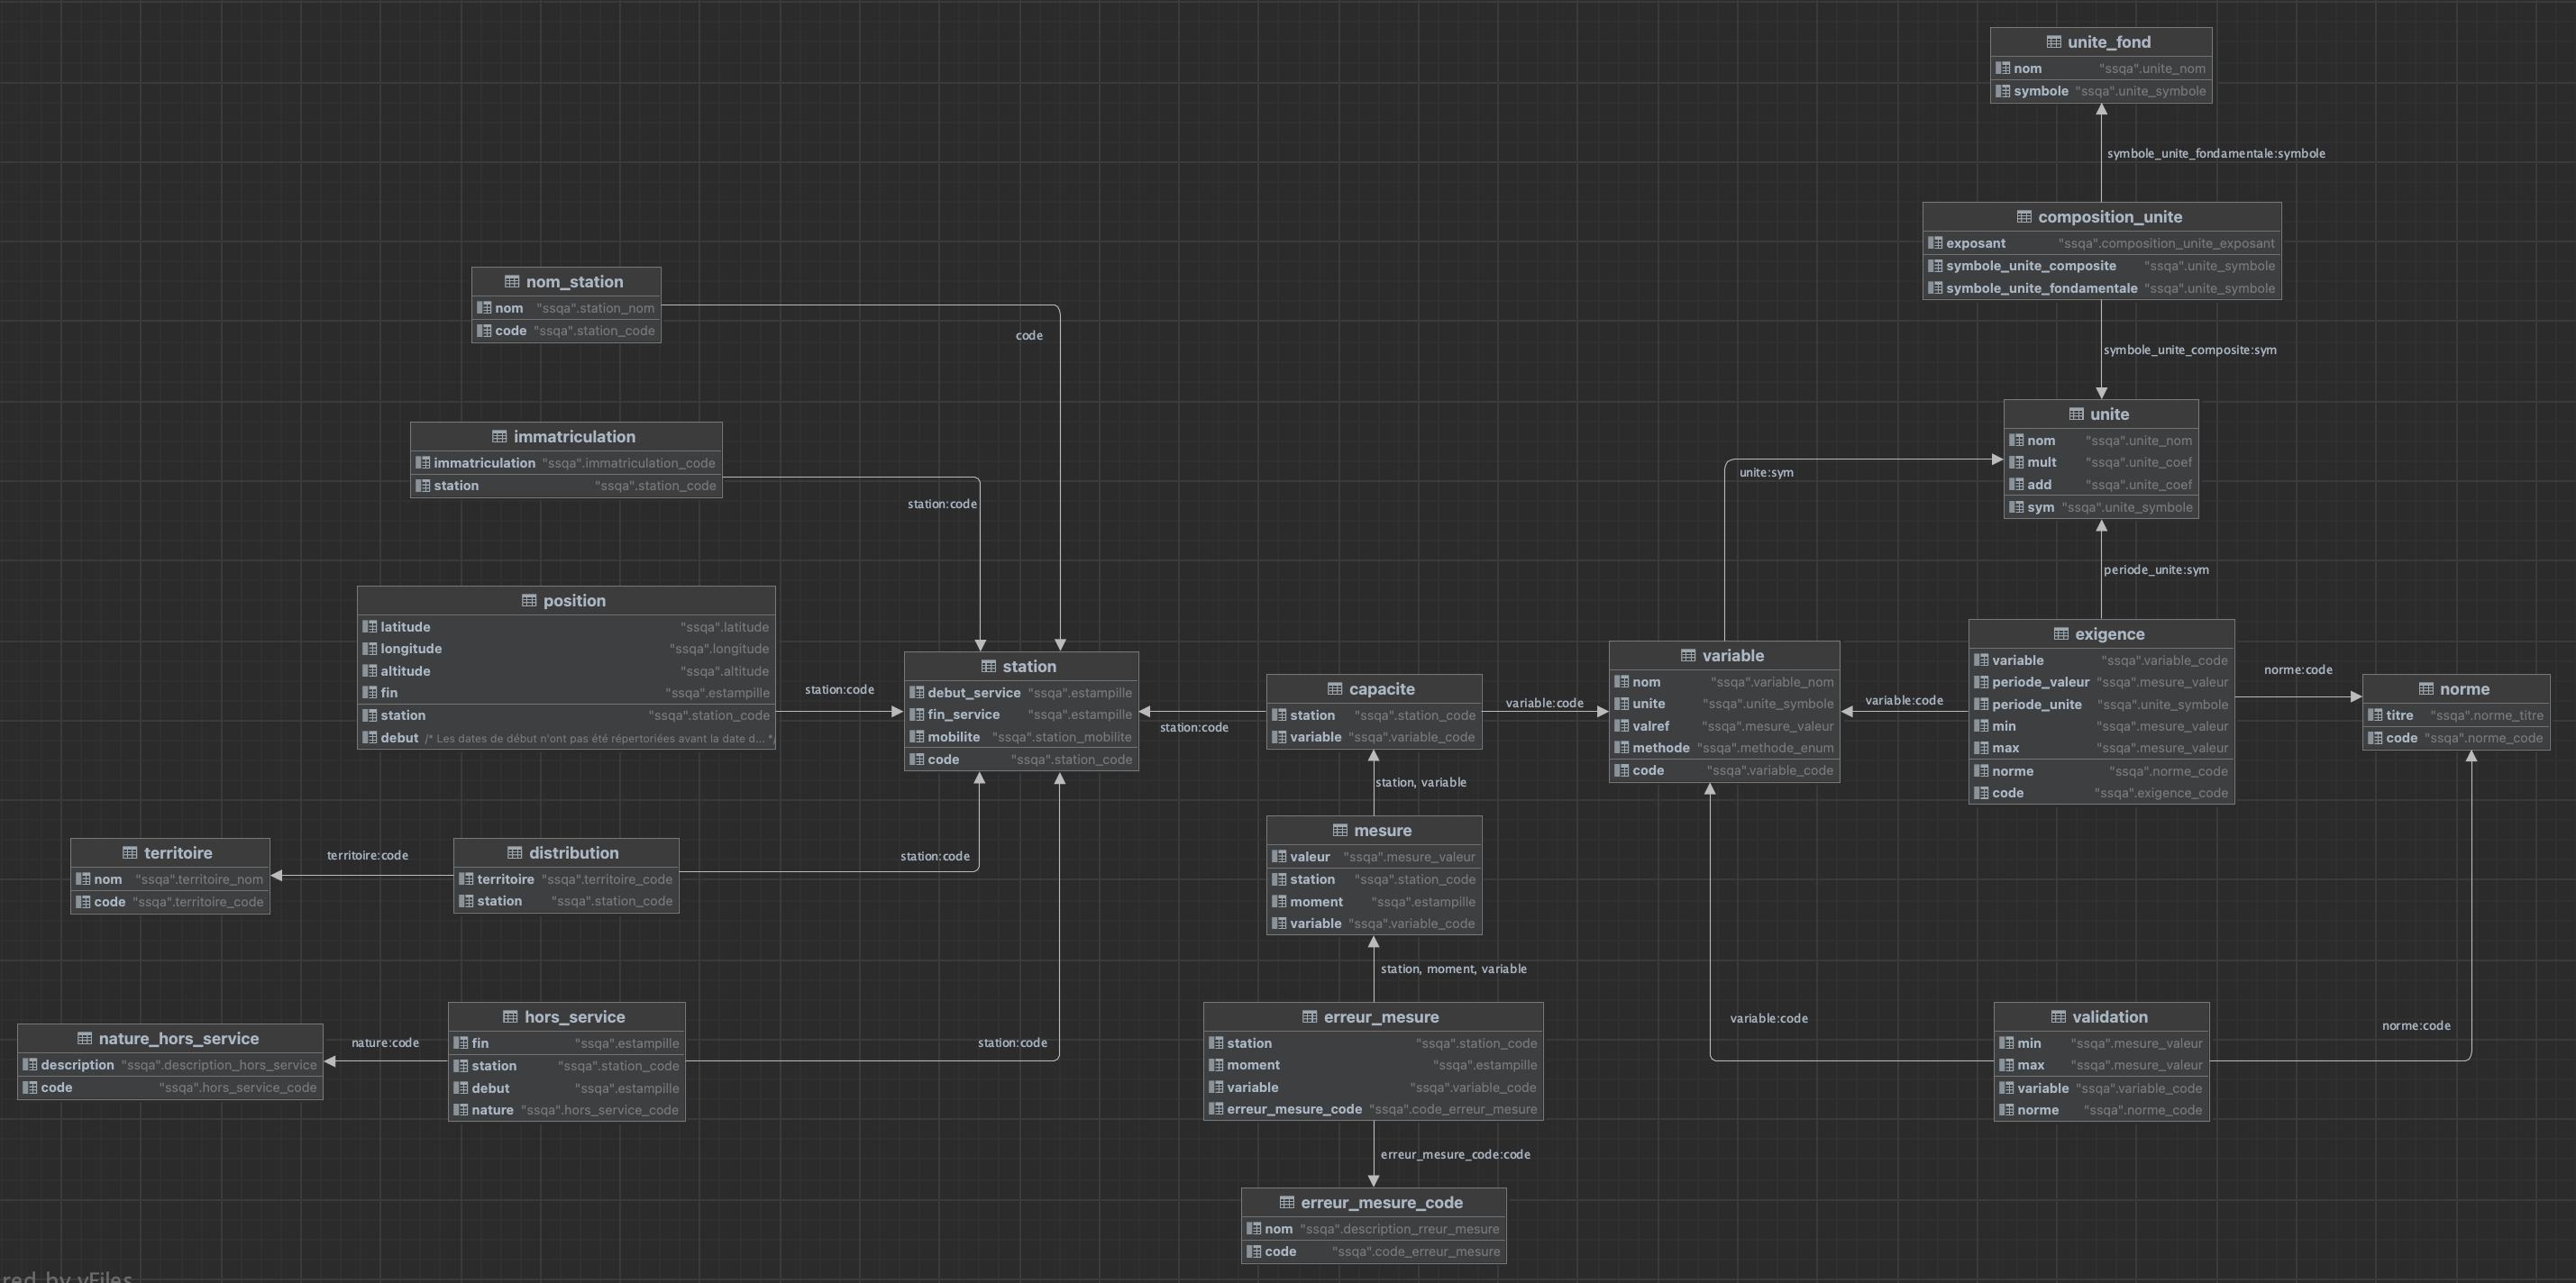
\includegraphics[width=1\textwidth]{db_modif.png}
    \caption{Schéma final de la base de données}
\end{figure}

\subsection{Système existant}
Le système existant est une base de données PostgreSQL correspondante
au schéma modifié ci-dessus. Les scripts de création de la base de données préliminaire
ont été fournis par le client et nous y avons ajouté des scripts qui
permettent la modification de la base de données en cours d'exploitation
pour implémenter les nouvelles fonctionnalités exigées par le jalon 1.

Il existe également une API permettant d'effectuer des opérations sur la base de données
et de récupérer les résultats de requêtes. Cette API contient les primitives
fondamentales d'évaluation, de modification, d'insertion et de retrait (ÉMIR) ainsi que
quelques fonctions plus complexes qui illustrent des cas d'utilisation typiques par le client.

\section{Problème}
Ce jalon porte sur la mise en place d'une base de données
analytique dimensionnelle (entrepôt de données) et sur l'implémentation
de son alimentation à partir de deux bases de données relationnelles.

\section{Exigences fonctionnelles}
\subsection{Création de l'entrepôt de données}
L'entrepôt de données doit prendre la forme d'un nouveau schéma dans 
la base de données PostgreSQL existante.

\subsection{Tables de faits}
L'entrepôt de données doit inclure au moins deux processus et leurs tables
de faits associées, choisis parmi les quatre processus explicités en cours.
Ces tables doivent également être accompagnées des tables de dimensions
correspondantes.

\subsection{Intégration des données de plusieurs sources}
L'entrepôt de données doit être alimenté par les données de la base de données
existante, mais également par les données provenant d'une autre base de données
compatible.

\subsection{Peuplement de l'entrepôt de données}
L'entrepôt de données doit être peuplé automatiquement à partir de l'API
de chacune des bases de données relationnelles intégrées.
Pour ce faire, certaines procédures ÉMIR de l'API existante devront être modifiées
afin de permettre l'insertion des données dans l'entrepôt.

\end{document}
